%%
%% This is file `sample-manuscript.tex',
%% generated with the docstrip utility.
%%
%% The original source files were:
%%
%% samples.dtx  (with options: `all,proceedings,bibtex,manuscript')
%% 
%% IMPORTANT NOTICE:
%% 
%% For the copyright see the source file.
%% 
%% Any modified versions of this file must be renamed
%% with new filenames distinct from sample-manuscript.tex.
%% 
%% For distribution of the original source see the terms
%% for copying and modification in the file samples.dtx.
%% 
%% This generated file may be distributed as long as the
%% original source files, as listed above, are part of the
%% same distribution. (The sources need not necessarily be
%% in the same archive or directory.)
%%
%%
%% Commands for TeXCount
%TC:macro \cite [option:text,text]
%TC:macro \citep [option:text,text]
%TC:macro \citet [option:text,text]
%TC:envir table 0 1
%TC:envir table* 0 1
%TC:envir tabular [ignore] word
%TC:envir displaymath 0 word
%TC:envir math 0 word
%TC:envir comment 0 0
%%
%% The first command in your LaTeX source must be the \documentclass
%% command.
%%
%% For submission and review of your manuscript please change the
%% command to \documentclass[manuscript, screen, review]{acmart}.
%%
%% When submitting camera ready or to TAPS, please change the command
%% to \documentclass[sigconf]{acmart} or whichever template is required
%% for your publication.
%%
%%
\documentclass[manuscript,screen]{acmart}

% Core for drawing
\usepackage{tikz}
\usetikzlibrary{arrows.meta,positioning,shapes.geometric,fit}
% pgfplots (the plotting package on top of TikZ)
\usepackage{pgfplots}
\pgfplotsset{compat=1.18}

\usepackage{booktabs}
%%
%% \BibTeX command to typeset BibTeX logo in the docs
\AtBeginDocument{%
  \providecommand\BibTeX{{%
    Bib\TeX}}}

%% Rights management information.  This information is sent to you
%% when you complete the rights form.  These commands have SAMPLE
%% values in them; it is your responsibility as an author to replace
%% the commands and values with those provided to you when you
%% complete the rights form.
\setcopyright{none}

%%
%% end of the preamble, start of the body of the document source.
\begin{document}

%%
%% The "title" command has an optional parameter,
%% allowing the author to define a "short title" to be used in page headers.
\title{Evaluation of Intermediate Steps in Retrieval Augmented Generation}

\author{Aram Aytekin}
\affiliation{%
  \institution{Universität Kassel}
  \country{Germany}}
\email{uk097201@student.uni-kassel.de}

\author{Moritz Dietrich}
\affiliation{%
  \institution{Universität Kassel}
  \country{Germany}}
\email{uk097299@student.uni-kassel.de}

\author{Maximilian Bennedik}
\affiliation{%
  \institution{Universität Kassel}
  \country{Germany}}
\email{uk095879@student.uni-kassel.de}

\author{Domenic Bremmer}
\affiliation{%
  \institution{Universität Kassel}
  \country{Germany}}
\email{uk095482@student.uni-kassel.de}


%%
%% By default, the full list of authors will be used in the page
%% headers. Often, this list is too long, and will overlap
%% other information printed in the page headers. This command allows
%% the author to define a more concise list
%% of authors' names for this purpose.
\renewcommand{\shortauthors}{Bremmer et al.}

%%
%% The abstract is a short summary of the work to be presented in the
%% article.
\begin{abstract}
This work investigates the research question: Does a RAG pipeline that expands the initial prompt into an LLM-generated query pool produce answers that humans prefer (on correctness, conciseness, and relevance) over a baseline that directly queries Elasticsearch once? To explore this, we implement two retrieval-augmented generation (RAG) pipelines that operate exclusively on search engine result page (SERP) snippets, which are often incomplete and inconsistent. The baseline pipeline (P1) retrieves snippets from a single query and directly conditions an LLM on this evidence. The advanced pipeline (P4), in contrast, employs LLM-based query expansion to generate a pool of reformulated queries, filters the resulting snippets, and integrates them for answer inference. Human evaluation indicates that P4 produces answers that are slightly more coherent, contextually appropriate, and preferred overall, though the improvements remain moderate. However, these gains come at the cost of significantly longer execution time, highlighting a trade-off between answer quality and system efficiency. These findings demonstrate the potential of query-expansion-based RAG pipelines for enhancing answer quality from fragmented snippet collections, while also pointing to open challenges in efficiency, evidence integration, and domain adaptation.
\end{abstract}

%%
%% The code below is generated by the tool at http://dl.acm.org/ccs.cfm.
%% Please copy and paste the code instead of the example below.
%%
\begin{CCSXML}
\begin{CCSXML}
<ccs2012>
   <concept>
       <concept_id>10002951.10003317.10003338</concept_id>
       <concept_desc>Information systems~Retrieval models and ranking</concept_desc>
       <concept_significance>500</concept_significance>
       </concept>
   <concept>
       <concept_id>10002951.10003317.10003359</concept_id>
       <concept_desc>Information systems~Evaluation of retrieval results</concept_desc>
       <concept_significance>500</concept_significance>
       </concept>
   <concept>
       <concept_id>10010147.10010178.10010179</concept_id>
       <concept_desc>Computing methodologies~Natural language processing</concept_desc>
       <concept_significance>300</concept_significance>
       </concept>
 </ccs2012>
\end{CCSXML}

\ccsdesc[500]{Information systems~Retrieval models and ranking}
\ccsdesc[500]{Information systems~Evaluation of retrieval results}
\ccsdesc[300]{Computing methodologies~Natural language processing}

%%
%% Keywords. The author(s) should pick words that accurately describe
%% the work being presented. Separate the keywords with commas.
\keywords{RAG, Summary, Pooling, Query, LLM, Pipeline}

%\received{20 February 2007}
%\received[revised]{12 March 2009}
%\received[accepted]{5 June 2009}

%%
%% This command processes the author and affiliation and title
%% information and builds the first part of the formatted document.
\maketitle

\section{Introduction}
\label{sec:introduction}

Information retrieval and answer generation have been transformed in recent years by large language models (LLMs) and retrieval-augmented generation (RAG). While these approaches typically rely on access to the full underlying documents, many real-world scenarios such as search engines only provide access to fragmented snippets contained in search engine result pages (SERPs). These snippets are often incomplete, inconsistent, and heterogeneous in style, making coherent answer generation particularly challenging. Nevertheless, being able to synthesize high-quality answers from such fragments is of both practical and theoretical interest.

A central obstacle in this setting lies in how queries are handled. Traditional retrieval methods issue a single query and directly return associated results, which often fails to capture the full breadth of relevant information. Recent advances in LLM prompting, however, allow for automatic query reformulation and expansion, potentially improving coverage and evidence diversity. Whether such query pooling strategies can indeed enhance answer generation quality from SERP snippets remains an open question.

	\subsection{Research Question}
	\label{subsec:research-question}
	Against this background, our study investigates the following research question: 
	\emph{Does a RAG pipeline that expands the initial prompt into an LLM-generated query pool produce answers that humans prefer (on correctness, conciseness, and relevance) over a baseline that directly queries Elasticsearch once?}
	
	\subsection{Contribution}
	\label{subsec:contribution}
	To answer this question, we implement and evaluate two RAG pipelines that operate solely on SERP snippets. The baseline pipeline (P1) issues a single query and generates answers from the retrieved snippets without further reformulation. The advanced pipeline (P4), in contrast, expands the initial query into a pool of reformulated queries using an LLM, retrieves and filters a broader snippet set, and conditions answer generation on this richer evidence. We evaluate both pipelines through human preference judgments along correctness, conciseness, and relevance, and further measure computational cost. Our findings show that while P4 produces answers that are slightly more coherent and preferred overall, it incurs substantially higher runtime costs, highlighting a trade-off between answer quality and efficiency. This contribution provides insight into the potential and the limitations of query-expansion-based RAG pipelines when applied to fragmented snippet data.

\section{Background \& Related Work}
\label{sec:background}

	\subsection{Retrieval Augmented Generation}
	\label{subsec:retrieval-augmented-generation}
	Retrieval-Augmented Generation (RAG) has emerged as a powerful paradigm for combining the generative capabilities of large language models (LLMs) with external retrieval mechanisms to produce factually grounded answers. In typical RAG setups, queries are used to retrieve relevant documents or passages from a large corpus, which are then used to condition the LLM’s response \cite{izacard-grave-2021-leveraging,NEURIPS2020_6b493230}. This approach mitigates hallucinations often observed in standalone LLMs and enhances factual accuracy. Previous studies have demonstrated the effectiveness of RAG in settings such as open-domain question answering, summarization, and knowledge-intensive tasks \cite{karpukhin-etal-2020-dense,guu2020realmretrievalaugmentedlanguagemodel}. However, most prior work assumes access to complete and well-structured documents. In contrast, the present study operates under the more constrained setting of search engine result page (SERP) snippets, which are often fragmented, inconsistent, and incomplete. This constraint introduces unique challenges for coherent answer generation, motivating the exploration of advanced retrieval strategies.
	
	\subsection{Query Expansion vs. Single-Query Baselines}
	\label{subsec:query-expansion-vs-baseline}
	Traditional information retrieval systems often rely on a single-query approach, issuing one query to retrieve the top-k documents or passages. While computationally efficient, this strategy may fail to capture the full spectrum of relevant evidence, particularly in domains with heterogeneous or incomplete sources. Query expansion techniques aim to address this limitation by reformulating the initial query or generating multiple variant queries to improve coverage. Classical methods include pseudo-relevance feedback and relevance-based models, whereas more recent approaches leverage LLMs to generate paraphrases, sub-questions, or expanded queries tailored to the information need \cite{nogueira2020passagererankingbert,wang-etal-2023-query2doc}. The trade-off is evident: query expansion can increase evidence diversity and retrieval effectiveness, but at the cost of additional computation and potential introduction of irrelevant information. In our study, the baseline pipeline (P1) represents the single-query approach, while the advanced pipeline (P4) operationalizes LLM-driven query expansion within a RAG framework, allowing for a systematic evaluation of this trade-off.

	\subsection{Human Preference Evaluation}
	\label{subsec:human-preference-eval}
	Automatic evaluation metrics such as BLEU \cite{post-2018-call}, ROUGE \cite{lin-2004-rouge}, and BERTScore \cite{zhang2020bertscoreevaluatingtextgeneration} are limited in their ability to capture the quality of open-ended answers, especially in terms of correctness, conciseness, and relevance \cite{karpukhin-etal-2020-dense}. Human evaluation remains the gold standard for assessing answer quality in generative tasks \cite{bai2022traininghelpfulharmlessassistant,thoppilan2022lamdalanguagemodelsdialog}. Pairwise preference judgments, where annotators compare outputs from different systems, have been widely adopted to obtain robust insights into model performance \cite{stiennon2022learningsummarizehumanfeedback}. 
	
	Recent work has shown that crowdsourcing can be a viable approach for evaluating RAG systems, enabling structured assessments while controlling for annotator variability \cite{Gienapp_2025}. Despite the advantages, human evaluation remains resource-intensive. In our study, we conduct a structured human preference evaluation comparing answers generated by P1 and P4 along three dimensions: correctness, conciseness, and relevance. This provides direct evidence of the practical impact of query pooling on perceived answer quality, complementing quantitative retrieval metrics and highlighting the cost-quality trade-offs inherent in LLM-driven RAG pipelines.


\section{Methods}

	\subsection{Pipelines}
	\label{subsec:pipelines}
	
	In this project, we compare two retrieval-augmented generation pipelines that
	differ in how they formulate and execute search queries before producing an
	LLM-based answer.
	
	\paragraph{Pipeline 1: Direct Retrieval and Answering.}
	In this baseline approach, the system directly takes the user’s input prompt
	and submits it as a query to the Elasticsearch retriever. The retriever returns the top-$k$ relevant text
	snippets, which are then provided to the LLM together with a
	strict system instruction: the model must formulate its answer \emph{only based
	on the retrieved snippets}. This ensures that the output is grounded in the
	search results without additional query expansion or prompt reformulation.
	
	\begin{figure}[H] % or [htbp]
		\centering
		\resizebox{\textwidth}{!}{%
		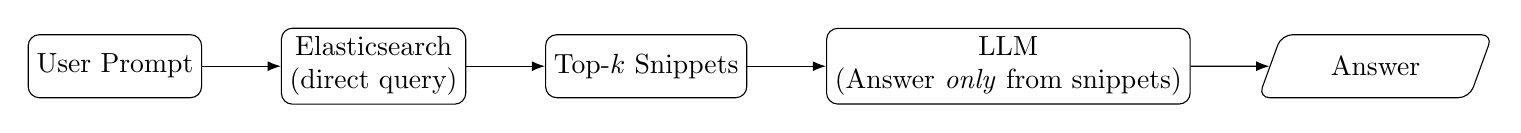
\begin{tikzpicture}[
		  node distance=7mm and 10mm, >=Latex,
		  box/.style={draw, rounded corners, align=center, minimum height=8mm, inner sep=3pt},
		  process/.style={box}, io/.style={box, trapezium, trapezium left angle=70, trapezium right angle=110}
		]
		\node[process] (p1_prompt) {User Prompt};
		\node[process, right=of p1_prompt] (p1_retr) {Elasticsearch\\(direct query)};
		\node[process, right=of p1_retr] (p1_snips) {Top-$k$ Snippets};
		\node[process, right=of p1_snips] (p1_llm) {LLM\\(Answer \emph{only} from snippets)};
		\node[io,      right=of p1_llm] (p1_out) {Answer};
		
		\draw[->] (p1_prompt) -- (p1_retr);
		\draw[->] (p1_retr) -- (p1_snips);
		\draw[->] (p1_snips) -- (p1_llm);
		\draw[->] (p1_llm) -- (p1_out);
		\end{tikzpicture}%
		}
		\caption{Pipeline~1 — direct retrieval from Elasticsearch and grounded answering from retrieved snippets.}
		\label{fig:pipeline1}
	\end{figure}
	
	\paragraph{Pipeline 4: Query Pool Expansion.}
	This enhanced approach adds an intermediate reasoning step before retrieval.
	The LLM is first asked to generate a \emph{query pool}, i.e.\ a set of
	reformulated or semantically related search queries derived from the original
	user prompt. These multiple queries are then executed against Elasticsearch,
	leading to a richer and more diverse set of retrieved snippets. The snippets
	are aggregated and passed to the LLM, which produces the final answer. By
	broadening the retrieval space, Pipeline~4 aims to increase coverage and
	relevance compared to the single-query baseline.
	
	\begin{figure}[H]
		\centering
		\resizebox{\textwidth}{!}{%
		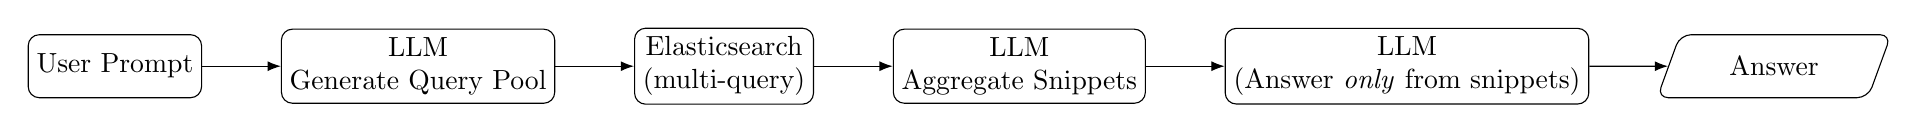
\begin{tikzpicture}[
		  node distance=7mm and 10mm, >=Latex,
		  box/.style={draw, rounded corners, align=center, minimum height=8mm, inner sep=3pt},
		  process/.style={box}, io/.style={box, trapezium, trapezium left angle=70, trapezium right angle=110}
		]
		\node[process] (p4_prompt) {User Prompt};
		\node[process, right=of p4_prompt] (p4_qpool) {LLM\\Generate Query Pool};
		\node[process, right=of p4_qpool] (p4_retr) {Elasticsearch\\(multi-query)};
		\node[process, right=of p4_retr] (p4_snips) {LLM\\Aggregate Snippets};
		\node[process, right=of p4_snips] (p4_llm) {LLM\\(Answer \emph{only} from snippets)};
		\node[io,      right=of p4_llm] (p4_out) {Answer};
		
		\draw[->] (p4_prompt) -- (p4_qpool);
		\draw[->] (p4_qpool) -- (p4_retr);
		\draw[->] (p4_retr) -- (p4_snips);
		\draw[->] (p4_snips) -- (p4_llm);
		\draw[->] (p4_llm) -- (p4_out);
		\end{tikzpicture}%
		}
		\caption{Pipeline~4 — LLM-generated query pool, multi-query retrieval, snippet aggregation, and grounded answering.}
		\label{fig:pipeline4}
	\end{figure}



	\subsection{Retrieval configuration}
	\label{subsec:retrieval-config}
	
	\paragraph{Data.}
	We retrieve over an Elasticsearch index built from the \emph{Archive Query Log (AQL-22)}~\citep{reimer:2023}, a corpus of archived search engine result pages (SERPs) containing historical queries and their snippet-level results (titles, snippets, target URLs). Crucially, because these SERPs are captured from the Internet Archive, the queries and their retrieved contexts are \emph{reproducible}; unlike commercial engines (e.g., Google) whose indices and ranking algorithms change over time, AQL provides a stable snapshot that makes our comparative analysis possible.
	
	\paragraph{Source retriever.}
	Our retriever queries the AQL-backed Elasticsearch index to collect snippet contexts that ground LLM answers. In \textbf{Pipeline~1}, the user prompt is issued as a single ES query; we take the top-$k$ snippets and pass them to the LLM with an instruction to answer \emph{only} from those snippets. In \textbf{Pipeline~4}, the LLM first generates a pool of reformulated queries; we execute each against the same index, merge and deduplicate the returned snippets, then feed the aggregated context to the LLM. Both pipelines operate on the identical index and use the same $k$ and filtering/cleanup steps to isolate the effect of the query strategy itself.


	
	\subsection{LLM Configuration}
	\label{subsec:llm-config}
	
	\subsection{Evaluation Protocol}
	\label{subsec:eval-protocol}
	xxx
	
	\subsection{Metrics \& Hypotheses}
	\label{subsec:metrics-hypo}
	
		
	\subsection{Cost Measurement}
	\label{subsec:cost-measure}
	
	
\section{Results}
\label{sec:results}

	\subsection{Overall Preference}
	\label{subsec:preference}
	
	% Figure: Winrate
	\begin{figure}[H]
	\centering
	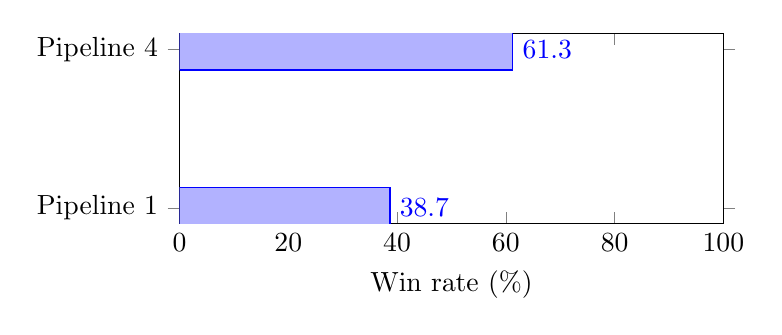
\begin{tikzpicture}
	\begin{axis}[
	  xbar,
	  width=0.7\textwidth,
	  height=4cm,
	  xlabel={Win rate (\%)},
	  xmin=0, xmax=100,
	  symbolic y coords={Pipeline 1,Pipeline 4},
	  ytick=data,
	  nodes near coords,
	  nodes near coords align={horizontal},
	  bar width=15pt,
	]
	\addplot coordinates {(38.7,Pipeline 1) (61.3,Pipeline 4)};
	\end{axis}
	\end{tikzpicture}
	\caption{Win rate comparison between Pipeline 1 and Pipeline 4.}
	\end{figure}

	
	\subsection{Annotator Remarks}
	\label{subsec:annotator-remarks}
	
	\subsection{Cost-Quality Tradeoff}
	\label{subsec:cost-quality-tradeoff}
	
	% Figure: line plot of mean time per question (1..20)
	\begin{figure}[H]
	\centering
	\begin{tikzpicture}
	\begin{axis}[
	  width=\textwidth,
	  height=0.5\textheight,
	  xlabel={Question (qid)},
	  ylabel={Mean time (s)},
	  xmin=1, xmax=20,
	  xtick={1,...,20},
	  ymajorgrids, xmajorgrids,
	  legend style={at={(0.5,1.05)},anchor=south,legend columns=-1},
	  enlarge x limits=0.02,
	  unbounded coords=jump, % <-- prevents interpolation over NaNs
	]
	
	% Pipeline 1
	\addplot+[
	  mark=*,
	  thick,
	  color=blue,           % <-- force distinct color
	  y filter/.code={%
	    \edef\p{\thisrow{pipeline}}%
	    \ifnum\pdfstrcmp{\p}{Pipeline 1}=0
	      % keep value
	    \else
	      \def\pgfmathresult{nan}% hide non-matching rows
	    \fi
	  }
	] table[
	  x=qid, y=mean_time_seconds, col sep=comma
	]{data/rag_time_long.csv};
	\addlegendentry{Pipeline 1}
	
	% Pipeline 4
	\addplot+[
	  mark=square*,
	  thick,
	  color=red,            % <-- force distinct color
	  y filter/.code={%
	    \edef\p{\thisrow{pipeline}}%
	    \ifnum\pdfstrcmp{\p}{Pipeline 4}=0
	      % keep value
	    \else
	      \def\pgfmathresult{nan}%
	    \fi
	  }
	] table[
	  x=qid, y=mean_time_seconds, col sep=comma
	]{data/rag_time_long.csv};
	\addlegendentry{Pipeline 4}
	
	\end{axis}
	\end{tikzpicture}
	\caption{Mean LLM response times per question (s) for the two pipelines.}
	\end{figure}

	
	\subsection{Annotator Remarks}
	\label{subsec:annotator-remarks}
	
	Annotators compared two anonymous answers for each prompt and selected the
	better one according to three criteria. The primary dimension was
	\textbf{Correctness}, i.e., factual accuracy, avoidance of hallucinations, and
	consistency with the question. Secondary criteria were:
	
	\begin{itemize}
	  \item \textbf{Relevance}: whether the answer stays on-topic and addresses the prompt,
	  \item \textbf{Conciseness}: whether the response is complete yet compact, without unnecessary repetition.
	\end{itemize}
	
	The evaluation followed a strict priority order:
	\textbf{Correctness} $\rightarrow$ \textbf{Relevance} $\rightarrow$
	\textbf{Conciseness}. When criteria conflicted, annotators were instructed to
	prefer the answer that was more accurate and cautious, even if it was less
	polished. If both answers were equally good (or equally poor), annotators could
	indicate \emph{No preference}.
	
	After each vote, annotators briefly justified their decision with a short
	comment referring to the criteria (e.g., correctness of facts, conciseness, or
	topicality). Critical errors or omissions were expected to be highlighted in
	these remarks.
	
	Finally, annotators were reminded to judge only the written content itself:
	unsupported or incorrect claims were to be penalized more heavily than cautious
	ones, and external searches were not permitted. Stylistic polish or formatting
	was not to influence voting unless it directly affected clarity.

	
	\subsection{Cost-Quality Tradeoff}
	\label{subsec:cost-quality-tradeoff}
	xxx
	
\section {Conclusion}
xxx


%%
%% The acknowledgments section is defined using the "acks" environment
%% (and NOT an unnumbered section). This ensures the proper
%% identification of the section in the article metadata, and the
%% consistent spelling of the heading.
\begin{acks}
To Robert, for the bagels and explaining CMYK and color spaces.
\end{acks}

%%
%% The next two lines define the bibliography style to be used, and
%% the bibliography file.
\bibliographystyle{ACM-Reference-Format}
\bibliography{cites}


%%
%% If your work has an appendix, this is the place to put it.
\appendix

\section{Research Methods}

\subsection{Part One}

Lorem ipsum dolor sit amet, consectetur adipiscing elit. Morbi
malesuada, quam in pulvinar varius, metus nunc fermentum urna, id
sollicitudin purus odio sit amet enim. Aliquam ullamcorper eu ipsum
vel mollis. Curabitur quis dictum nisl. Phasellus vel semper risus, et
lacinia dolor. Integer ultricies commodo sem nec semper.

\subsection{Part Two}

Etiam commodo feugiat nisl pulvinar pellentesque. Etiam auctor sodales
ligula, non varius nibh pulvinar semper. Suspendisse nec lectus non
ipsum convallis congue hendrerit vitae sapien. Donec at laoreet
eros. Vivamus non purus placerat, scelerisque diam eu, cursus
ante. Etiam aliquam tortor auctor efficitur mattis.

\section{Online Resources}

Nam id fermentum dui. Suspendisse sagittis tortor a nulla mollis, in
pulvinar ex pretium. Sed interdum orci quis metus euismod, et sagittis
enim maximus. Vestibulum gravida massa ut felis suscipit
congue. Quisque mattis elit a risus ultrices commodo venenatis eget
dui. Etiam sagittis eleifend elementum.

Nam interdum magna at lectus dignissim, ac dignissim lorem
rhoncus. Maecenas eu arcu ac neque placerat aliquam. Nunc pulvinar
massa et mattis lacinia.

\end{document}
\endinput
%%
%% End of file `sample-manuscript.tex'.
